\chapter{Instrumentação Industrial}

A instrumentação diz respeito aos intrumentos para medição, monitoração e controle de sistemas. Corresponde, grosso modo, ao nível 0 da pirâmide de automação, sem contar os atuadores.

Em geral, se estudam os atuadores separadamente, em disciplinas ou livros dedicados a motores elétricos, sistemas fluido-mecânicos, entre outros, de onde instrumentação industrial fica mais restrita aos sensores e dispositivos de interface humana mais simples, que é o que trata este capítulo. 
\section{nomenclatura}

A partir da definição do que trata a instrumentação, as funções dos equipamentos -- os instrumentos --  são: 
\begin{itemize}
  \item medição de variáveis -- sensores,
  \item indicação de valores e/ou condições a operadores -- indicadores,
  \item registro de dados dos sensores -- registradores, 
  \item transmissão de dados entre os dispositivos -- transmissores, 
  \item controle e comando do processo idustrial -- dispositivos de interface humana, como chaves, botões, \emph{sliders}, etc.
\end{itemize} 

Logo de início, há dois termos de significado próximo: sensor e transdutor. A definição destes termos está longe de ser uma unanimidade, com significados diferentes em diferentes áreas. Do ponto de vista da instrumentação, define-se:

\begin{quote}
  Sensor é um elemento que gera um sinal padronizado (normalmente elétrico, mas pode ser pneumático ou de outro tipo) a partir de uma grandeza física (calor, luz, som pressão etc).
\end{quote}
\begin{quote}
  Transdutor é um dispositivo que converte um sinal de uma grandeza para outra.
\end{quote}

Destas definições se conclui que todo sensor é um transdutor, mas não o contrário. Em geral os sensores se utilizam de transdutores para converter uma grandeza específica para outra mais facilmente manipulável. Dizendo de outro modo, todo sensor precisa ter um elemento transdutor, que não necessáriamente está no mesmo corpo que o sensor.

Uma classificação bastante útil é separando o tipo de sáida dos sensores, entre discretos ou contínuos:

\begin{description}
  \item[Sensores discretos] geram uma saída discretizada, normalmente binária --- 0 ou 1, aberto ou fechado, acionado ou desligado.
  \item[Sensores contínuos] geram uma saída que varia continuamente em função da entrada. Pode ser composto por um único transdutor (um resistor por exemplo).
\end{description}

Um complicador é que alguns textos técnicos e alguns ambientes fabris confundem estes termos, chamando sensores discretos simplesmente de sensores e sensores contínuos de transdutores. Portanto deve-se tomar cuidado com o significado destes termos em diferentes ambientes.

Do ponto de vista do fluxo de energia, pode-se classificar tanto sensores como transdutores como passivos ou ativos:
\begin{description}
  \item[Sensores ativos] geram um sinal de saída sem a necessidade de alimentação externa. Exemplos: termopar, célula fotoelétrica.
  \item[Sensores passivos] requerem uma entrada de energia para gerar um sinal de saída. Exemplos: Termorresistência, sensor capacitivo.
\end{description}

Esta classificação é menos útil no ambiente industrial, onde a maioria dos sensores são passivos, mesmo que internamente usem algum transdutor ativo.

\section{Sensores discretos}

Como citado, a maioria dos sensores discretos são binários. Além disto, a saída mais comum de um sensor binário industrial é na forma de uma chave elétrica, que pode estar aberta ou fechada. Neste caso diferenciam-se três categorias: os sensores de contato, acionados pelo contato com alguma coisa; os sensores de proximidade, que detectam a presença de algum objeto sem tocá-lo; e as chaves de processo, que atuam em função de uma variável do processo estar acima ou abaixo de determinado limiar.

\subsection{Sensores de contato}
Do ponto de vista da instrumentação, qualquer chave presente no nível 0 da pirâmide que gera sinais lidos no nível 1 realiza logicamente o mesmo tipo de função. Daí que se consideram como sensores de contato:
\begin{description}
  \item[Botoeiras] ou botões, acionados pelo operador do processo, mas que obviamente não são sensores no significado estrito do termo.
  \item[Chaves de fim de curso] que são acionadas mecanicamente por algo no processo.
\end{description}

As botoeiras podem ter diversos formatos e funções, vide a figura~\ref{fig:botoeiras}. Podem ser simples botões que fecham o contato apenas quando pressionados (sem retenção) do tipo liga e desliga (com retenção), interruptores de 3 estados, entre outros. Além disso é comum o uso de indicadores luminosos na própria botoeira.

Alguns botões de emergência são acionados quando apertados e precisam ser girados para destravarem e desligarem ou só são desligados com o uso de uma chave. Também é comum botoeiras que energizam equipamentos poderem ser travadas na posição desligada com um cadeado, o que permite que o manutentor trave o equipamento desenergizado enquanto efetua algum serviço.

\begin{figure}
  \centering
  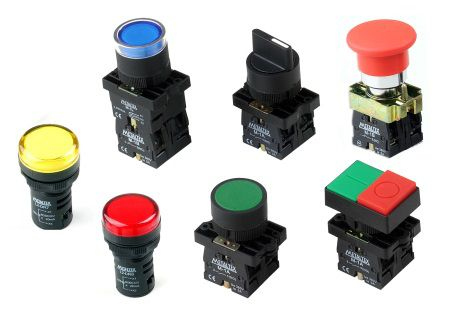
\includegraphics[width=0.6\textwidth]{figuras/botoeiras}
  \caption{Diversos tipos de botoeiras.}\label{fig:botoeiras}
\end{figure}

Chaves de fim de curso são chaves eletromecânicas feitas para serem acionadas por algum produto ou equipamento. São usadas para detectar, por exemplo, a passagem do material sendo processado por um determinado ponto, a posição final de movimentação de algum equipamento, entre outros. Normalmente é implementado como um botão com uma alavanca ou algum outro mecanismo na parte a ser acionada.

\begin{figure}
  \centering
  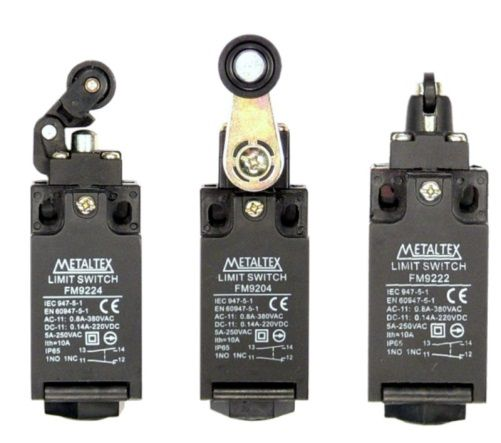
\includegraphics[width=0.6\textwidth]{figuras/fim-de-curso}
  \caption{Exemplos de chaves de fim de curso.}\label{fig:fim-de-curso}
\end{figure}

As chaves eletromecânicas são relativamente baratas, de uma tecnologia já bem amadurecida e praticamente imunes a interferências eletromagnéticas, porém o movimento a que são submetidas gera desgaste, o que faz com que sua vida útil seja reduzida. Além disso, necessitam do contato com o alvo para ser acionadas, o que pode ser inviável em alguns casos, e tem um tempo de resposta da ordem de milisegundos, que pode ser lento demais para algumas aplicações.

\subsection{Sensores de proximidade}

Um sensor de proximidade determina a presença de material em certa região próxima a ele sem a necessidade de tocar no material. Existem diversos princípios físicos que podem e são usados para tal fim. Estes sensores normalmente são aplicados quando se tem algum impedimento ao uso de chaves eletromecânicas ou em outras situações específicas ao tipo de sensor, quando o tipo de material a ser detectado é importante, por exemplo.

Para vários casos, é comum o uso de um encapsulamento em formato de rosca, como visto na figura \ref{fig:proximidade}. Isto faz com que vários sensores de proximidade se pareçam, mesmo que usem princípios físicos diferentes.

\begin{figure}
  \centering
  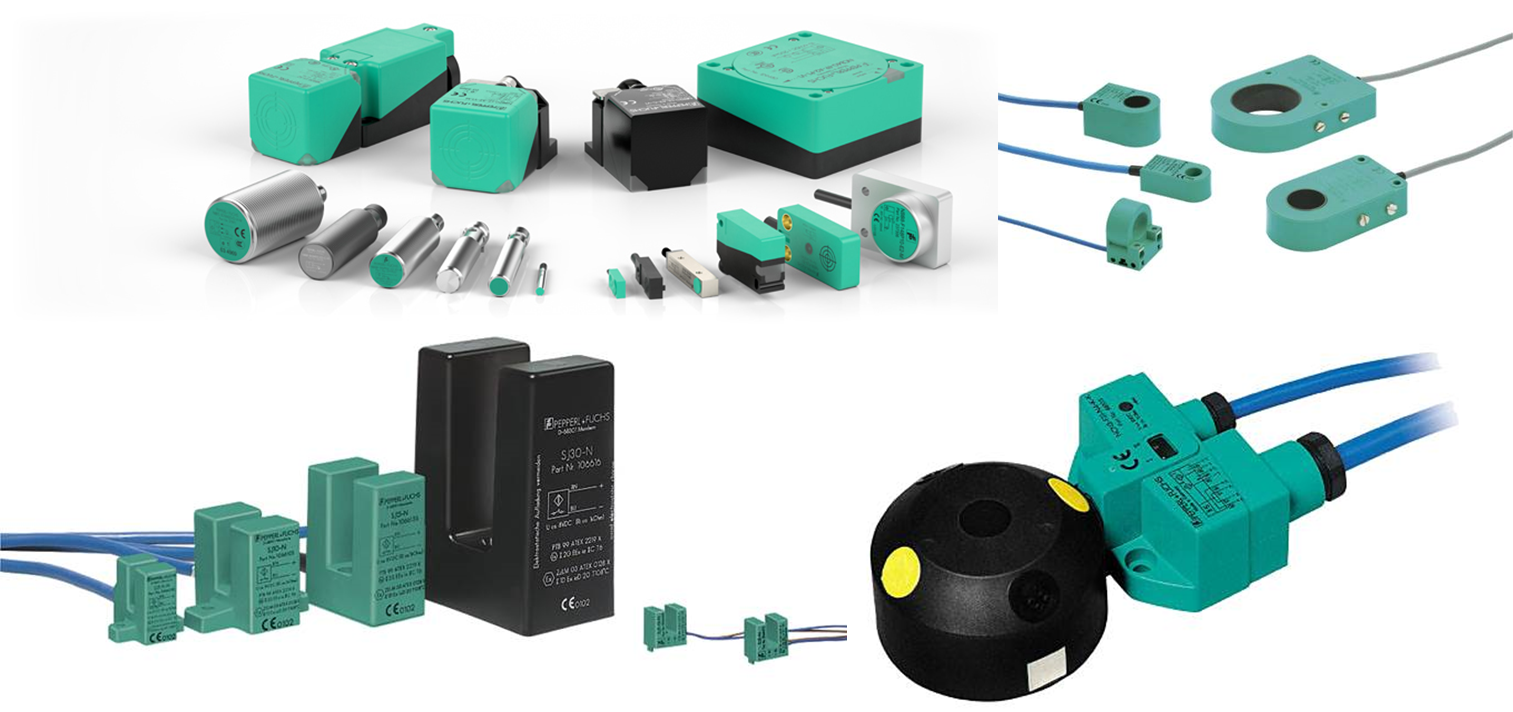
\includegraphics[width=0.9\textwidth]{figuras/Sensores-de-Proximidade_2}
  \caption{Encapsulamentos comuns para sensores de proximidade.}\label{fig:proximidade}
\end{figure}

Além do tipo, é possivel ter sensores de proximidade "blindados". Um sensor blindado faz com que o campo de atuação do sensor fique mais limitado à sua frente.

Os tpos mais comuns de sensores de proximidade industriais são o indutivo, o capacitivo e o óptico.

\subsubsection{Indutivo}
\label{subs:Indutivo}
O sensor indutivo conta com uma bobina na sua extremidade sensora, que gera um campo magnético variável na sua frente. A frequência deste campo magnético depende da própria indutância desta bobina, que por sua vez depende do que estiver na frente do sensor.

Um alvo que esteja na frente deste sensor pode alterar esta indutância por 2 efeitos: se for um condutor, gerará um campo magnético contrário por indução de correntes em seu meio, aumentando a indutância; se for ferroelétrico, concentrará o campo magnético, também aumentando a indutância. Como este segundo efeito é maior que o primeiro, este sensor é mais sensível a ferro do que a cobre, mesmo com o cobre sendo melhor condutor que o ferro.

A distância que um sensor indutivo consegue detectar um alvo de ferro na sua frente é chamada de \textbf{distância sensora nominal} - $Sn$. Para outros materiais esta distância sensora diminui e para materiais não condutores e sem propriedades magnéticas ela cai a zero. A figura \ref{fig:distancia_sensora} mostra a variação da distância sensora de sensores indutivos e capacitivos para diferentes materiais.

\begin{figure}
  \centering
  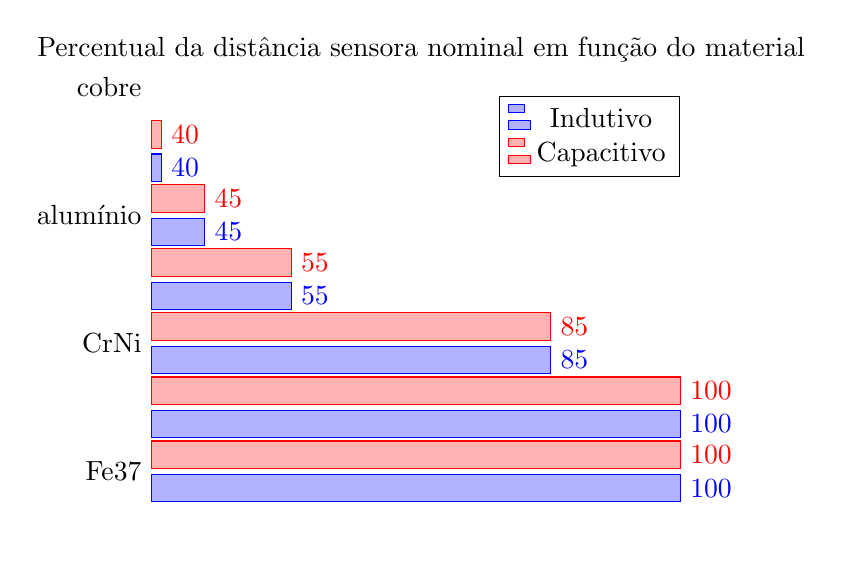
\begin{tikzpicture}
    \begin{axis}[title  = Percentual da distância sensora nominal em função do material,
      xbar,
      y axis line style = { opacity = 0 },
      axis x line       = none,
      tickwidth         = 0pt,
      enlarge y limits  = 0.2,
      enlarge x limits  = 0.02,
      symbolic y coords = {Fe37, Sae1020, CrNi, latão, alumínio, cobre },
      nodes near coords,
    ]
    \addplot coordinates { (100,Fe37) (100,Sae1020) (85,CrNi)  (55,latão) (45,alumínio) (40,cobre) };
    \addplot coordinates { (100,Fe37) (100,Sae1020) (85,CrNi)  (55,latão) (45,alumínio) (40,cobre) };
    %\addplot coordinates { (14320,LaTeX)         (1615,Tools)
    %                       (560,Distributions)   (3075,Editors)  };
    \legend{Indutivo,Capacitivo}
    \end{axis}
  \end{tikzpicture}
  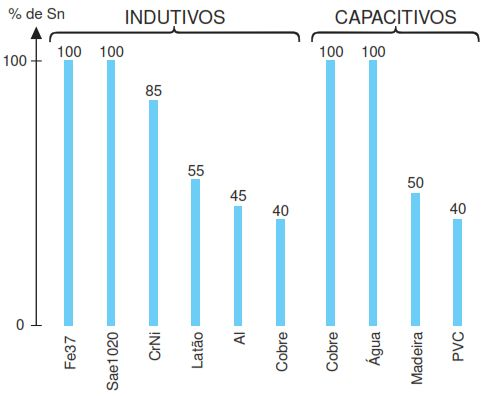
\includegraphics[width=0.6\textwidth]{figuras/distancia_sensora}
  \caption{Variação da distância sensora de sensores indutivos e capacitivos para diferentes tipos de material.}\label{fig:distancia_sensora}
\end{figure}

Além da limitação da distância que o sensor alcança, tipicamente abaixo de 10 cm, e da limitação do material do alvo, sensores indutivos estão sujeitos a interferências eletromagnéticas, que podem gerar falsas detecções.

\subsubsection{Capacitivo}
\label{subs:Capacitivo}

Sensores capacitivos usam um circuito oscilador (basicamente o mesmo de sensores indutivos) para detectar a variação da capacitância entre duas placas metálicas na sua ponta. Esta capacitância aumenta se o alvo tiver uma constante dielétrica maior que a do ar. Funciona muito bem para água e cobre (que tem uma constante dielétrica 80 vezes maior que o ar) e praticamente não responde para ferro, aço e alumínio.

Pela fraca sensibilidade a papel e plástico, pode detectar a presença de alguns objetos dentro da embalagem. Pela alta sensibilidade à água, é muito usado para detecção de nível, ao invês de um sensor tipo boia. Também é sensível à interferência eletromagnética, embora menos que o indutivo.

\subsubsection{Ultrassônico}
\label{subs:Ultrassonico}

Sensores ultrassônicos detectam a presença de um objeto pelo eco de um sinal ultrassônico (com frequência por volta de \SI{40}{kHz}). Também é muito usado para sensores contínuos de distância, já que o tempo do eco, ou seja, o tempo que o som demora para voltar, $t_e$ pode ser usado para determinar a distância até o alvo $d$ através de uma equação linear:
\begin{equation}
  d = \frac{1}{2}v_s t_e,
\end{equation}
onde $v_s$ é a velocidade do som. No uso como sensor contínuo deve-se tomar o cuidado de compensar a variação do $v_s$ com temperatura e pressão atmosférica.

Sensores ultrassônicos podem ser usados para detectar alvos em distâncias de até alguns metros, muito embora aí deva se ter o cuidado de que não haja outros elementos que possam gerar eco, por ter um cone de sensibilidade relativamente grande. É sensível não apenas à qualidade do material mas também à geometria do mesmo, quando pode perder o alvo completamente.

Outra limitação de sensores ultrassônicos é que eles tem uma distância mínima de trabalho. Se o alvo estiver muito próximo o sensor não consegue diferenciar o eco do sinal que ele ainda está gerando. Esta distância tipicamente está abaixo de 1 cm.

\subsubsection{Óptico}
\label{subs:optico}

Sensores ópticos funcionam com um emissor e um receptor de luz. Tipicamente se usa luz infravermelha, pois a eletrônica baseada em silício é mais sensível a este comprimento de onda, o que barateia o custo, mas em alguns casos se usa o vermelho quando se tem vantagem de ver onde a luz está chegando. Normalmente o sinal luminoso é modulado num trem de pulsos, para diminuir a interferência do sol, cuja luz contém infravermelho mas não é modulada. A implementação usual é com um led ou um laser de semicondutor como emissor e um fototransistor como receptor.

\begin{figure}
  \centering
  \subfloat[por reflexão]{\includegraphics[width=0.4\textwidth]{figuras/sensorOpticoReflexao}}
  \qquad
  \subfloat[por retro reflexão]{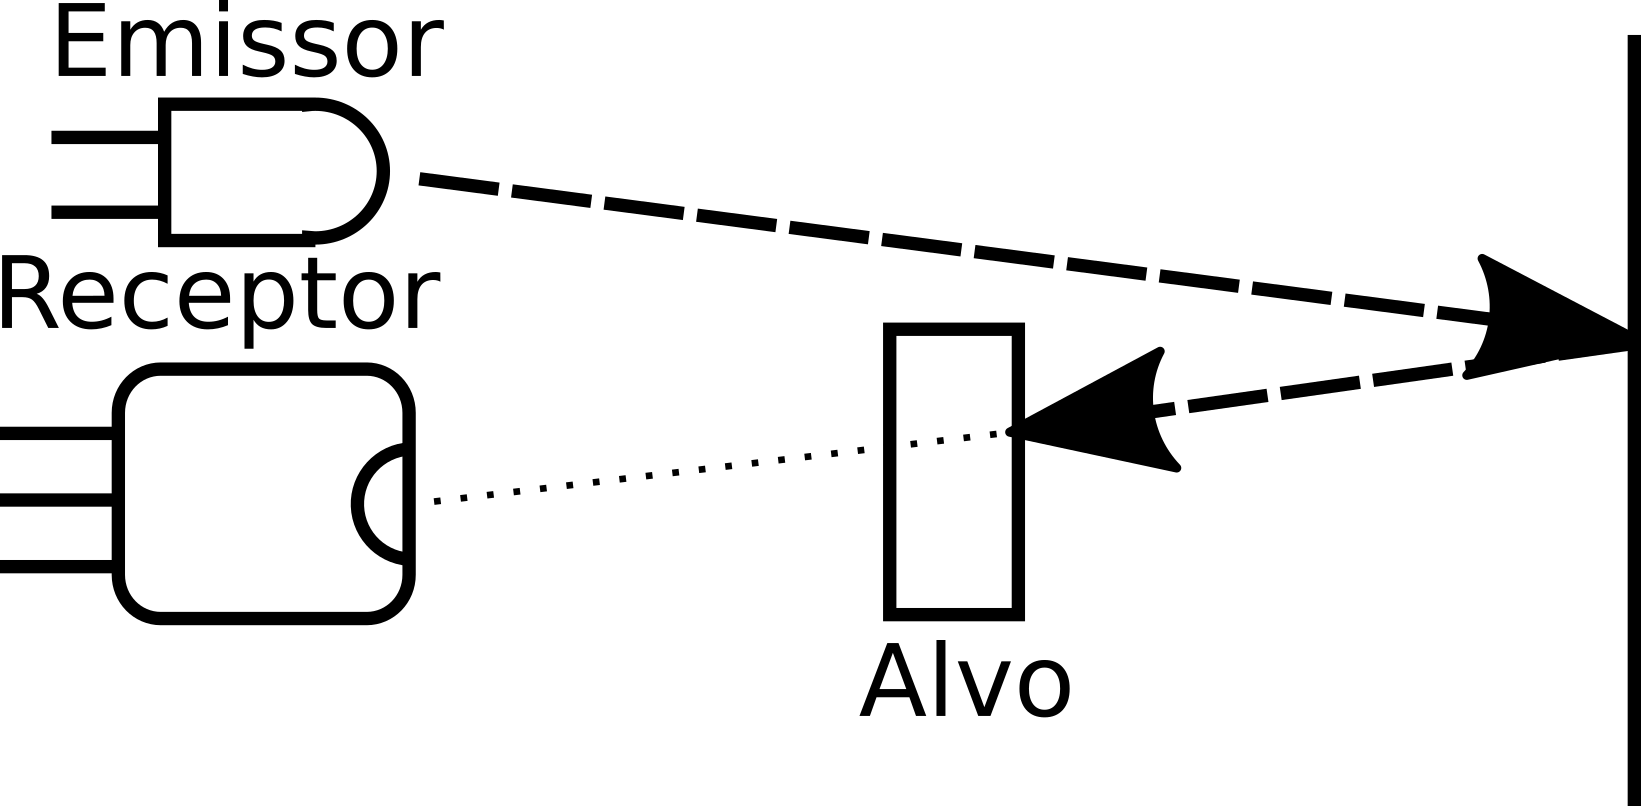
\includegraphics[width=0.4\textwidth]{figuras/sensorOpticoRetro}}

  \subfloat[por barreira]{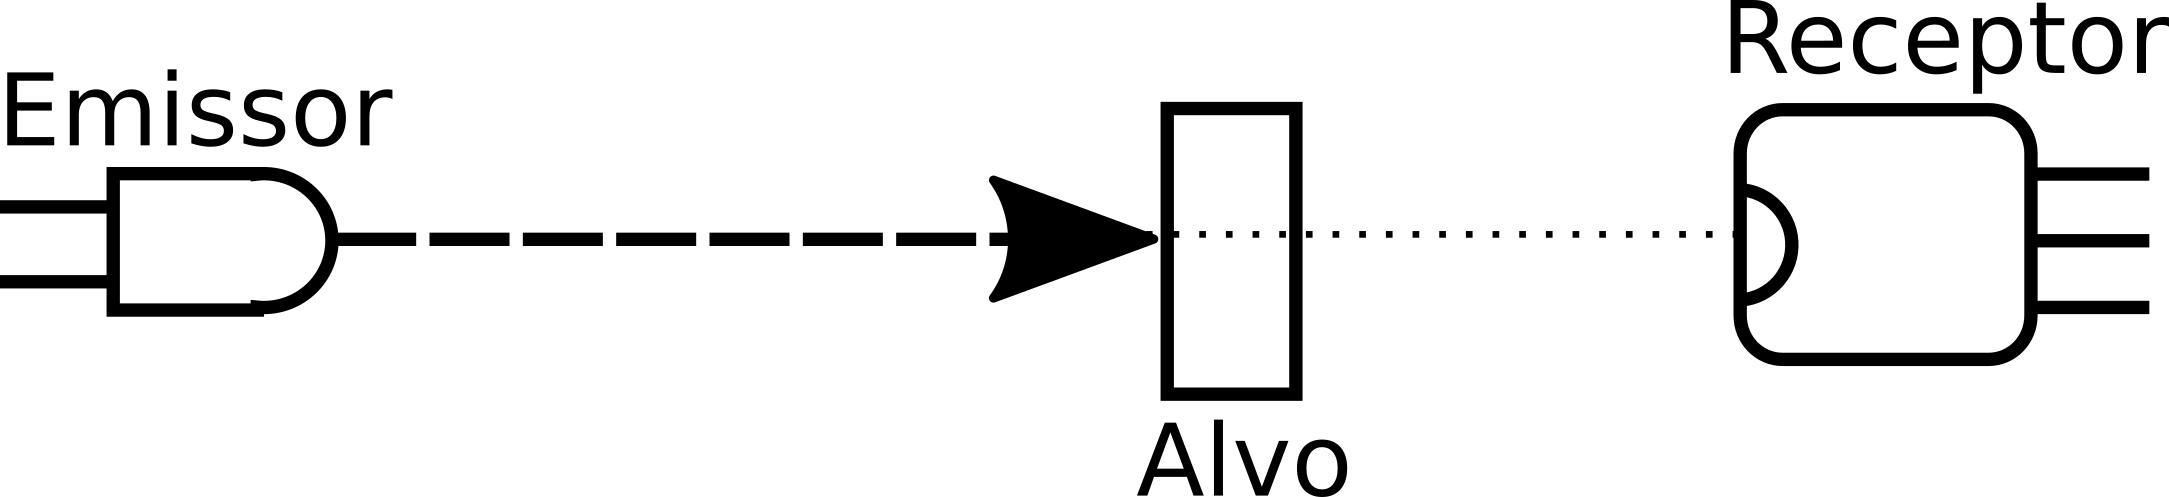
\includegraphics[width=0.4\textwidth]{figuras/sensorOpticoBarreira}}
  \caption{Princípio de funcionamento de diferentes configurações de sensor óptico.}\label{fig:sensorOptico}
\end{figure}

As configurações mais comuns deste tipo de sensor são:
\begin{description}
  \item[Por reflexão difusa] com o emissor do lado do receptor e detecta-se o alvo pelo seu reflexo. É o método usado na maioria dos \emph{smart phones} para detectar que o usuário está com o telefone no ouvido e desligar a tela. Figura \ref{fig:sensorOptico}a.
  \item[Por retro reflexão] que é o mesmo caso mas com um anteparo reflexivo atrás. Neste caso o alvo impede a passagem da luz. Figura \ref{fig:sensorOptico}b.
  \item[Por barreira] que usa o emissor e receptor separados e detecta-se a oclusão do feixe óptico. O uso de um laser como emissor permite alcançar uma grande distância. Figura \ref{fig:sensorOptico}c.

  Um uso interessante do sensor óptico de barreira é a chamada barreira laser, onde um conjunto de lasers passando por espelhos cercam um equipamento mais perigoso, de modo que qualquer pessoa ou coisa que acione a barreira enquanto o equipamento está atuando cause uma parada de emergência, diminuindo o risco do equipamento.
\end{description}

Além da luz ser imune a influência eletromagnética, o uso de fibras ópticas pode separar bastante a eletrônica do processo, permitindo o uso deste tipo de sensor em regiões onde não pode ter equipamentos elétricos, seja por excessivo ruído eletromagnético do processo seja por risco de explosão.

\subsubsection{Magnético}
\label{subs:Magnetico}

Há dois tipos básicos de sensores magnéticos: sensores Hall e \emph{reed switches}. Ambos detectam a presença de um campo magnético, normalmente causado pela aproximação de um imã.

O sensor Hall detecta o campo magnético pela influência do mesmo numa corrente elétrica -- o chamado efeito Hall. É muito usado para medir a rotação em eixos com um imã acoplado ou em motores elétricos. É um sensor barato, de alta durabilidade e rápido tempo de resposta, porém apenas aplicável a alvos magnetizados.

O \emph{reed switch} é composto de dois contatos de material ferromagnético normalmente separados, tal como mostra a figura \ref{fig:reed}. Um campo magnético perpendicular a estes contatos causam a magnetização dos mesmos, o que faz com que eles se atraiam e fechem contato.

\begin{figure}
  \centering
  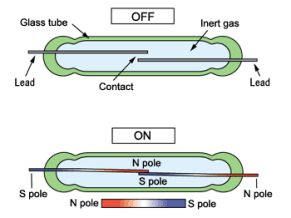
\includegraphics[width=0.5\textwidth]{figuras/reed}
  \caption{\emph{Reed Switch}.}\label{fig:reed}
\end{figure}

O \emph{reed switch} é bem mais barato que o Hall, mas tem pouca durabilidade e elevado tempo de resposta.

\subsection{Chaves de processo}

Chaves de processo são chaves elétricas que atuam quando uma grandeza do processo de fabricação (uma variável de processo) passa determinado nível. Por exemplo: temperatura do tanque 1 acima de \SI{100}{\celsius}, nível do silo abaixo de \SI{2}{\meter}, e assim por diante.

São exemplos de chaves de processo:
\begin{description}
  \item[bóias] que acionam um contato elétrico,
  \item[sensor capacitivo] acionado pelo nível de água de um reservatório,
  \item[chaves de fluxo] onde uma lingueta aciona uma chave eletromecânica se o fluxo passar de um  determinado limite,
  \item[termostatos] que acionam quando a temperatura passa de determinado nível, entre outros.
\end{description}

É cada vez mais comum trocar as chaves de processo por sensores contínuos e implementar o limite de chaveamento por software no controlador. Isto permite uma maior flexibilidade, pois variar o limite no software é mais simples.

\section{Sensores Contínuos}

Sensores contínuos usam algum princípio físico para a medição de alguma grandeza física. As grandezas mais comumente medidas são temperatura, comprimento (nível, espessura, posição), vazão e pressão.

\subsection{Pressão e força}
\label{sub:Pressão e força}
Como pressão é força por área, se se consegue medir um, pode-se usar o mesmo princípio físico para medir outro.

Os principais princípios físicos para a medição de pressão ou força são:
\begin{description}
  \item[Coluna de líquido] que usa um tubo fino com um líquido. Ao se colocar o tubo de ponta cabeça, o líquido escorre deixando um vácuo. O comprimento do vácuo é proporcional à pressão externa.

  Normalmente se usa como um indicador. Não é adequado para interfacear com circuitos elétricos.

  \item[Deformação elástica] que utiliza a deformação de um elemento elástico -- normalmente um metal por conta da durabilidade -- para determinar a pressão. O elemento elástico em si pode ter vários formatos: formato de C, helicoidal, espiral, diafragma.

Pode ser usado tanto como mero indicador, acoplando o elemento elástico a um ponteiro (medidor Bordon tipo C, por exemplo), ou como um transdutor acoplado a uma fita extensiométrica.

  \item[Piezorresistência] é a variação da resistência com a tração ou compressão usada na fita extensiométrica, também conhecida por \emph{strain gage}. Ao ser colado a um elemento elástico, permite transformar a deformação deste elemento num sinal elétrico. É bastante usada em balanças eletrônicas e também no monitoramento de estruturas metálicas.

  \item[Piezoelétricidade] é o efeito apresentado por alguns cristais (normalmente se usa o quartzo) que geram um sinal elétrico ao serem submetidos a uma força e geram uma força quando lhe são aplicados sinais elétricos. Isto permite a construção de circuitos osciladores que variam a sua frequência de ressonância natural em função da força aplicada.
\end{description}

\subsection{Temperatura}
Entre as diversas maneiras de medir temperatura, destacam-se:
\begin{description}
  \item[Tubo capilar], também conhecido como termômetro líquido. Usa um líquido que ao sofrer expansão térmica ocupa um tubo capilar, que permite visualizar a temperatura. Bom para visualização mas não adequado para automação, por não sr fácil gerar um sinal elétrico a partir dele.

  \item[Termopar] Pode-se determinar a energia necessária para retirar elétrons de um determinado camada, o que se chama de \emph{função trabalho} do material. Quando dois materiais diferentes se juntam, a diferença da função trabalho deles gera um potencial elétrico. Normalmente este potencial elétrico não é percebido pois ao se fazer um circuito fechado de diferentes materiais com todas as junções na mesma temperatura, estas diferenças acabam se anulando. Porém, se pegarmos dois fios condutores com diferentes funções trabalhos,unirmos uma ponta e colocarmos esta junção numa temperatura diferente, como num forno, por exemplo, aparece uma tensão que é função dos materiais usados e da diferença de temperatura. Este é o chamado efeito Seebeck:
  \[
E = (S_\mathrm{B} - S_\mathrm{A}) \cdot (T_2 - T_1),
  \]
  onde E é a tensão gerada, $S_\mathrm{A}$ e $S_\mathrm{B}$ são os coeficientes de Seebeck dos materiais A e B e $T_2$ e $T_1$ são as temperaturas nas diferentes junções.

Logo o termopar mede a diferença de temperatura entre dois lugares e não a temperatura absoluta, precisando de um medidor auxiliar para medir a temperatura ambiente.

Existem diversos tipos de termopar, formados por diferentes junções de metais. Há vários tipos padrões identificados por uma letra: J - ferro e constantan; K - Níquel-Cromo e Níquel-Alumínio; S - Platina e Ródio e Platina. Escolhe-se o tipo pela faixa de operação, precisão e custo. A tabela \ref{tab:termopares} mostra a faixa de operação e precisão de alguns tipos de termopar.

\begin{table}
  \caption{Características de diversos tipos de termopar.}
  \label{tab:termopares}
  \begin{tabular}{ccccc}
    \hline
    Tipo J & Tipo K & Tipo R & Tipo S & Tipo T\\
    \hline
    \SI{0}{\celsius} a \SI{760}{\celsius}  & \SI{0}{\celsius} a \SI{1370}{\celsius} & \SI{0}{\celsius} a \SI{1000}{\celsius} & \SI{0}{\celsius} a \SI{1750}{\celsius} & \SI{-160}{\celsius} a \SI{400}{\celsius} \\
    \SI{\pm 0,1}{\celsius} & \SI{\pm 0,7}{\celsius} &\SI{\pm 0,5}{\celsius} &\SI{\pm 1,0}{\celsius} &\SI{\pm 0,5}{\celsius} \\
    \hline
  \end{tabular}
\end{table}

\item[Delta de tensão de junções] -- pode-se usar dois transistores bipolares para gerar uma diferença de tensão ($\Delta V_{BE}$) que é proporcional à temperatura absoluta (em Kelvin). É limitado à faixa de temperatura em que a eletrônica funciona: de aproximadamente \SI{-55}{\celsius} a \SI{120}{\celsius}.

O grande uso da eletrônica fez com que o custo deste tipo de dispositivo caísse bastante, principalmente quando integrado em algum outro circuito. É muito usado em termômetros digitais, no controle de temperatura de processadores de computador e na compensação da temperatura ambiente em circuitos de medição de termopares.

  \item[Termorresistor] utiliza a variação da resistência de um condutor com a temperatura. Usa um polinômio que relaciona a resistência com a temperatura, como:
  \[
R = R_0[1+a\cdot T+b\cdot T^2],
  \]
onde T é a temperatura em Celsius e $R_0$ é a resistência quando a temperatura é de \SI{0}{\celsius}.

São usados metais inertes, tais como o níquel ou a platina. O nome do sensor é o símbolo do elemento químico usado seguido do valor de $R_0$ em Ohms: Pt100, Ni500, etc.

\item[Pirômetro] ou termômetro de infravermelho usa a chamada radiação do corpo negro para determinar a temperatura. Todo objeto emite fótons de comprimento de onda relacionado à temperatura do objeto. O pirômetro mede então o comprimento de onda destes fótons, permitindo a medição da temperatura à distância.

Apesar da praticidade ainda são bastante caros, embora o custo venha diminuindo rapidamente. Hoje se usam também as câmeras térmicas, baseadas no mesmo princípio.
\end{description}

\section{Características dos Instrumentos}
\label{sec:Características dos Instrumentos}

Podemos separar entre características estáticas e dinâmicas. As principais características estáticas são:
\begin{description}
  \item[Sensibilidade - S] Relação entre um acréscimo na grandeza medida ($x$) e o acréscimo correspondente na saída do sensor ($Y$).
  \[
S = \frac{\partial y}{\partial x}
  \]
Se a curva é uma reta, a sensibilidade é constante. Além disso, se o 0 da entrada gera 0 na saída, pode ser chamado de ganho.
\item[Faixa de Operação] Faixa de valores de entrada para a qual o dispositivo funciona. Também chamado de Faixa nominal.

Algumas vezes, a Faixa é referida como sendo a diferença entre o valor máximo e mínimo do instrumento.
\item[Faixa de Operação de Saída] Faixa de valores de saída gerados pelo dispositivo. Também chamado de Fundo de escala.

Se o instrumento for linear, pode-se tirar a seensibilidade a partir da faixa de operação de entrada e de saída.
\item[Resolução] Menor variação da entrada que gera uma variação na saída.

Para instrumentos digitais, está relacionado ao número de bits do conversor analógico-digital usado.
\item[Exatidão] O quanto o valor médio dado pelo instrumento corresponde ao valor real.
\item[Precisão] O quanto as medições variam em torno do valor médio.
\begin{figure}
 \centering
  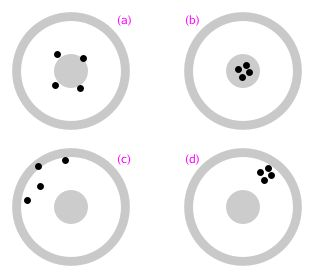
\includegraphics[width=0.6\textwidth]{figuras/precisaoExatidao}
  \caption{Representação de precisão e exatidão.a) Exato e Não Preciso. b) Exato e Preciso. c) Não Exato e Não Preciso. d) Não Exato e Preciso.}\label{fig:precisaoExatidao}
\end{figure}
\item[Repetibilidade] Capacidade do instrumento de reproduzir as mesmas saídas quando as mesmas entradas são aplicadas, sob as mesmas condições.
É calculado como sendo a amplitude máxima observada nas medições de saída em relação à faixa de operação de saída.
\[
\text{Repetibilidade} = \frac{y_{max}-y{min}}{\text{Faixa de operação de saída}}
\]
\item[Reprodutibilidade] Grau de concordância entre os resultados das medições de uma mesma grandeza, onde as medições individuais são efetuadas variando-se uma ou mais das seguintes condições:
\begin{itemize}
  \item Método de medição.
  \item Instrumento de medida.
  \item Observador.
  \item Outras variáveis (temperatura, pressão, etc.).
\end{itemize}
\item[Não linearidade] O quanto o instrumento diverge de uma relação linear entre entrada e saída.

Normalmente é medido como a pior diferença entre a resposta do instrumento e a resposta linear.
\item[Histerese] Quando há diferentes saídas para uma mesma entrada,
conforme o valor da entrada for crescente ou decrescente.
\begin{figure}
  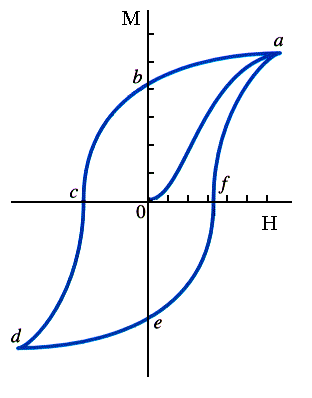
\includegraphics[width=0.6\textwidth]{figuras/histerese}
  \caption{Representação de histerese.}\label{fig:histerese}
\end{figure}
\item[Banda morta] Região onde não existe variação na saída para uma
determinada faixa de valores de entrada.
\begin{figure}
  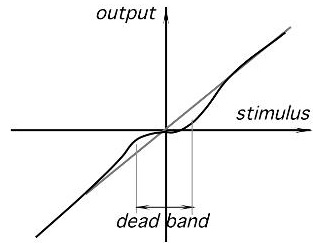
\includegraphics[width=0.6\textwidth]{figuras/bandamorta}
  \caption{Representação de banda morta.}\label{fig:bandaMorta}
\end{figure}
\end{description}

A resposta dinâmica do instrumento é relacionada a variação da saída ao longo do tempo em função da variação da entrada. Os principais parâmetros são:
\begin{description}
  \item[Velocidade de resposta] Medida pelo tempo que o instrumento demora para variar em função de uma mudança em degrau da entrada.
  \item[Atraso] O quanto o instrumento demora para fazer qualquer mudança após uma variação da entrada.
  \item[\emph{Overshoot}] O quanto a medida passa do valor final ao ter uma alteração da entrada.
  \item [Faixa de frequência] As frequências de entrada às quais o instrumento responde.
  \item[Desvio] O quanto a saída muda ao longo do tempo, mesmo se a entrada estiver parada.
\end{description}


% \section{Transmissão de dados, aterramento e blindagem em instrumentação.}
